\newpage
\section{Descrizione design pattern}
\subsection{Introduzione}
I \glo{Design pattern}{design pattern} semplificano l'attività di progettazione, favorendo il riutilizzo del codice e rendendo l'architettura più manutenibile. I design pattern vengono definiti come soluzioni progettuali generali a problemi ricorrenti. Si tratta di una descrizione o dei modelli logici da applicare per la risoluzione di problemi che possono presentarsi durante la \glo{Fase}{fase} di progettazione. Esistono diversi design pattern e vengono suddivisi in base al problema da risolvere:
\begin{itemize}
	\item \textbf{pattern creazionali}: nascondono i costruttori delle classi e espongono dei metodi al loro posto. In questo modo si possono utilizzare oggetti senza sapere come sono implementati;
	\item \textbf{pattern comportamentali}: forniscono soluzione alle più comuni tipologie di interazione tra gli oggetti;
	\item \textbf{pattern architetturali}: operano ad un livello più elevato rispetto ad altri design pattern, ed esprimono schemi di base per impostare l'organizzazione strutturale di un sistema software. In questi schemi si descrivono sottosistemi predefiniti, i ruoli che essi assumono e le relazioni reciproche;
	\item \textbf{pattern strutturali}: consentono di riutilizzare degli oggetti esistenti fornendo agli utilizzatori un'interfaccia più adatta alle loro esigenze.
\end{itemize}
Sono stati utilizzati i seguenti design pattern:
\begin{itemize}
	\item Factory Method (creazionale);
	\item Redux (architetturale).
\end{itemize}

Di seguito verranno mostrati i design pattern utilizzati e come vengono contestualizzati nel progetto \progetto{}. I diagrammi delle classi mostrati in queste comparazioni sono parziali e a scopo illustrativo. Per la loro visualizzazione completa si rimanda alla sezione \ref{componenti}.

\newpage
\subsection{Pattern Creazionali}

\subsubsection{Factory Method}
\paragraph{Descrizione}
Questo pattern permette di creare oggetti fornendo un'interfaccia per creare un oggetto, ma lascia che le sottoclassi decidano quale oggetto istanziare.
Il pattern factory può essere utilizzato quando:
\begin{itemize}
\item la creazione di un oggetto preclude il suo riuso senza una significativa duplicazione di codice.
\item la creazione di un oggetto richiede l'accesso ad informazioni o risorse che non dovrebbero essere contenute nella classe di composizione.
\item la gestione del \glo{Ciclo di vita}{ciclo di vita} degli oggetti gestiti deve essere centralizzata in modo da assicurare un comportamento coerente all'interno dell'applicazione.
\end{itemize}
\paragraph{Contestualizzazione}
Questo pattern viene utilizzato nel package \texttt{StorePkg::PolygonPkg}. Sono state create le classi \texttt{ConcretePolygon}, che implementa l'interfaccia \texttt{Polygon}, e \texttt{ConcretePolygonFactor}y, che implementa l'interfaccia \texttt{PolygonFactory}. \texttt{PolygonFactory} espone il metodo \texttt{CreatePolygon}, che viene sovrascritto dalla sua sottoclasse \texttt{ConcretePolygonFactory} consentendo quindi ai suoi utilizzatori, \texttt{Scenario} e \texttt{\glo{Asset}{Asset}}, la creazione dell'oggetto di tipo \texttt{Polygon}.
	\begin{figure}[H]
		\label{builder_compara}
		\centering
		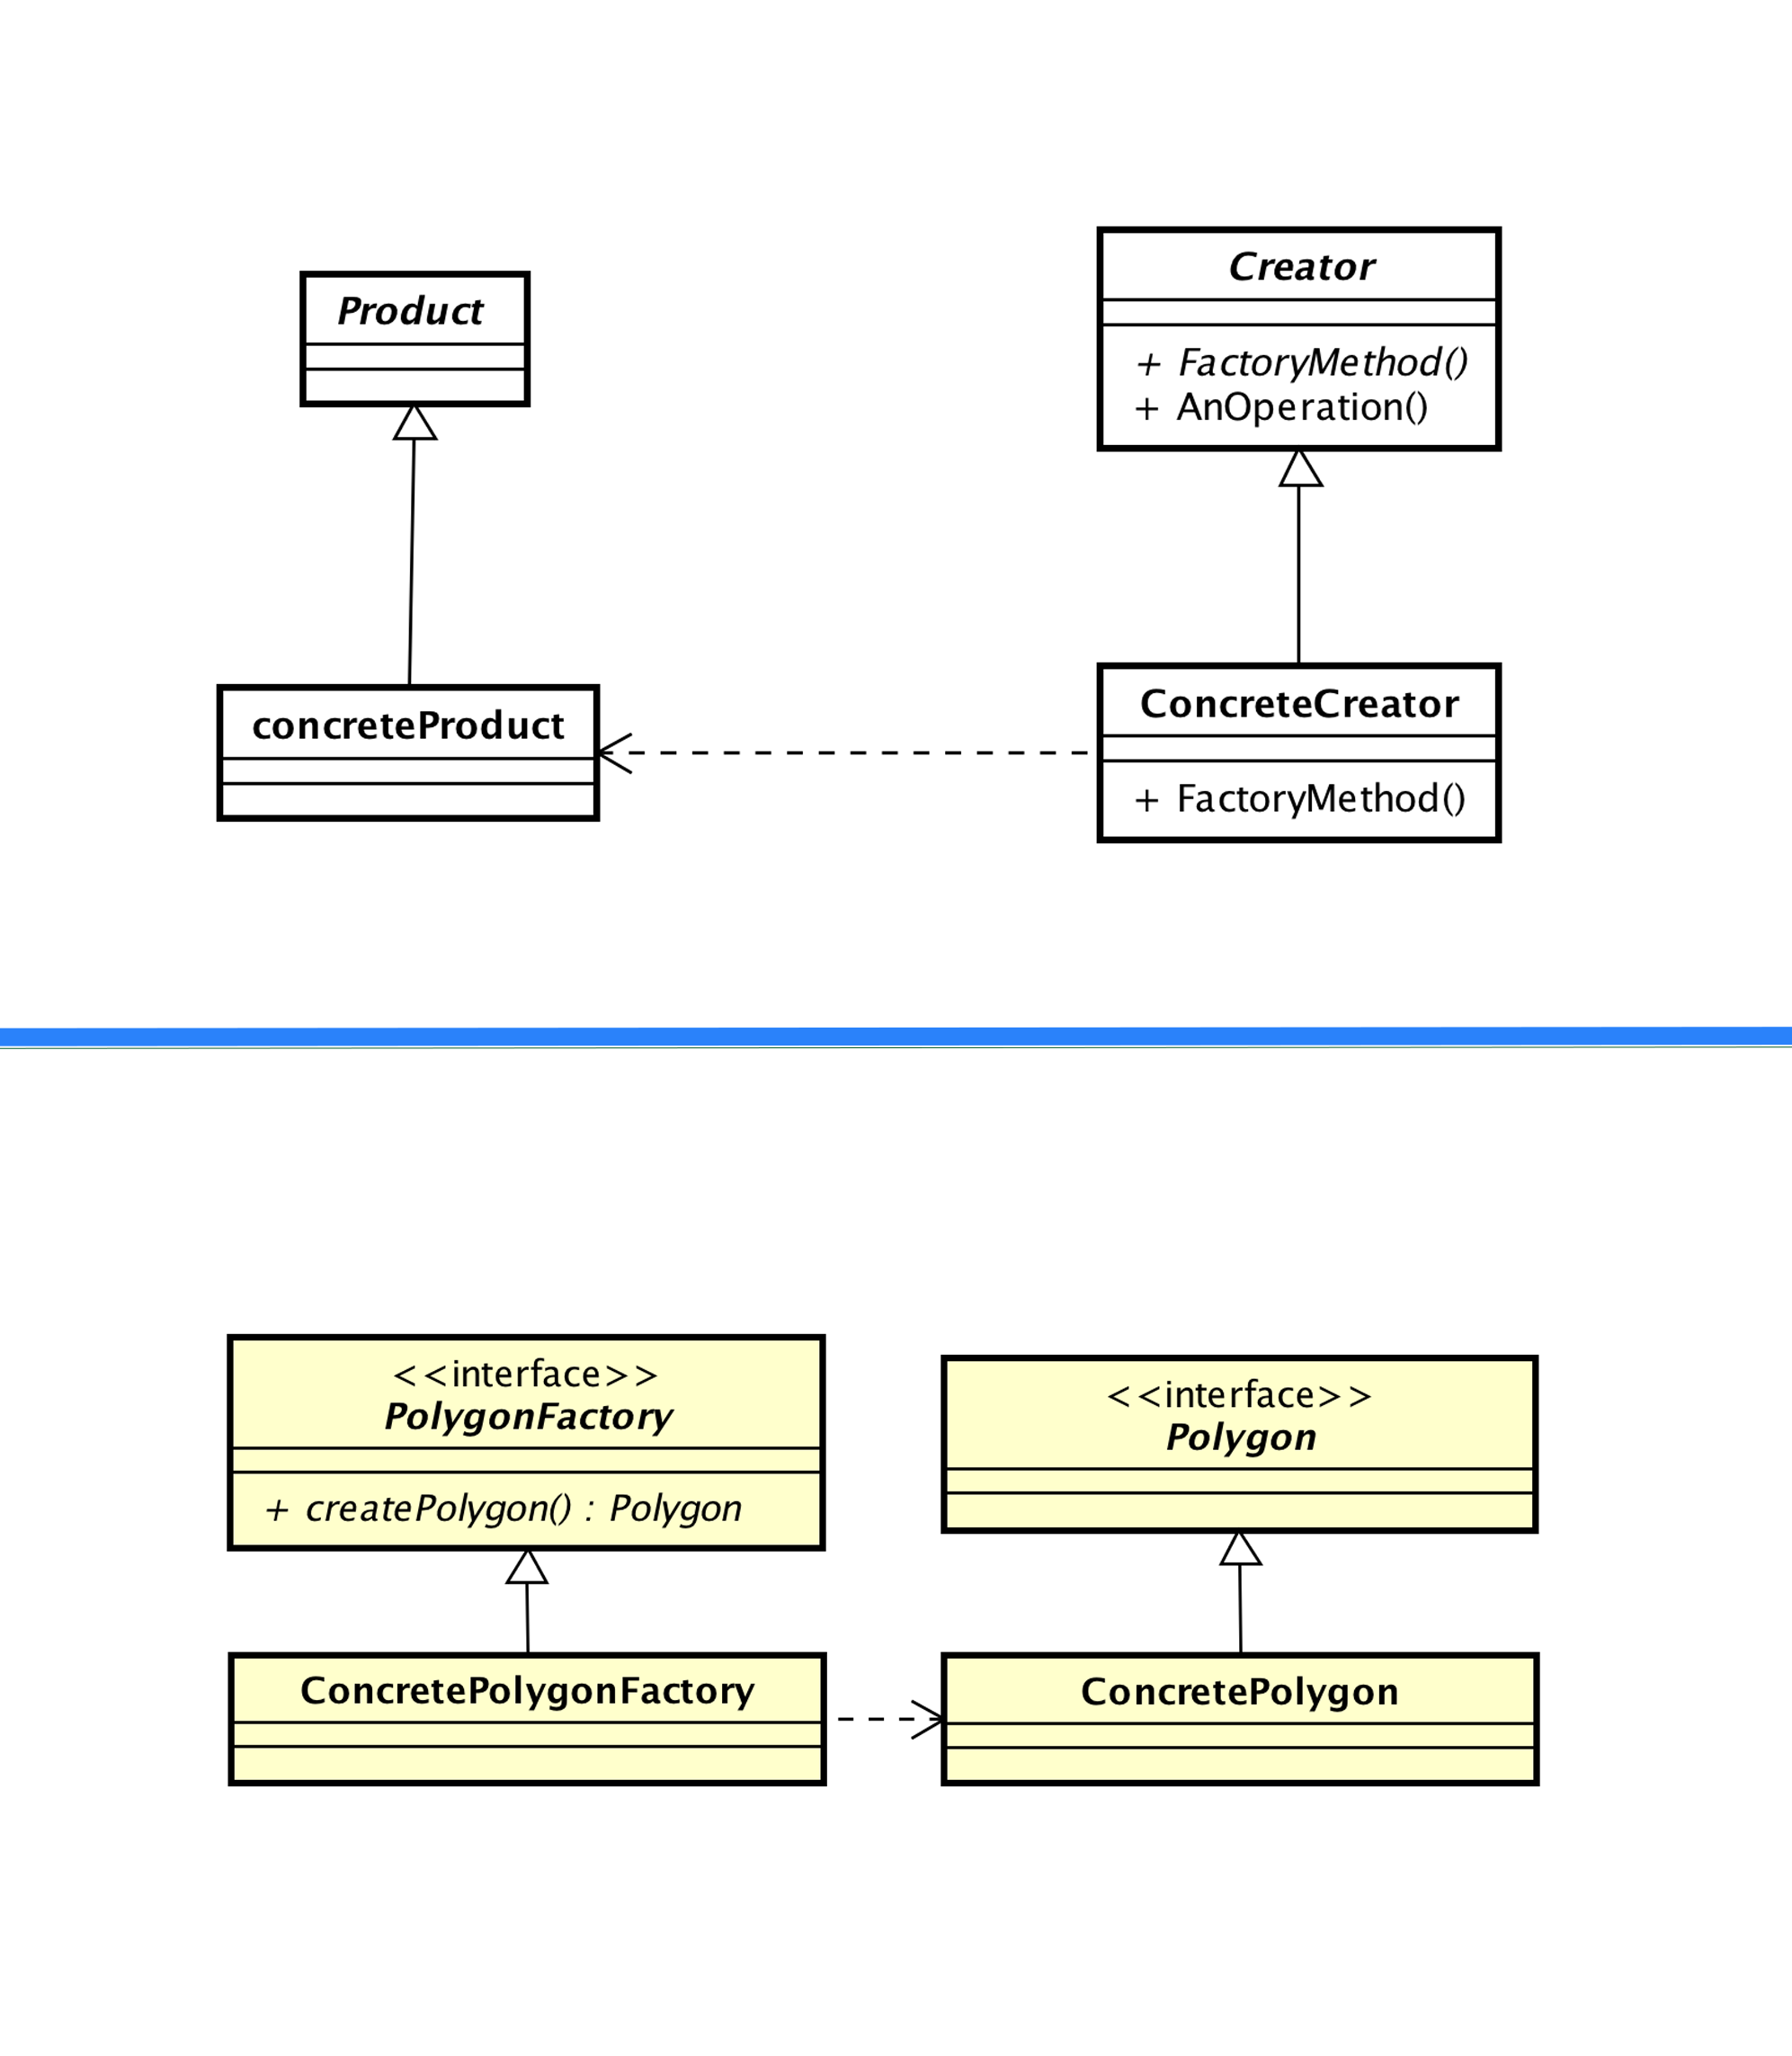
\includegraphics[scale=0.12]{img/factoryComparati.png}
		\caption{Factory Method e la sua contestualizzazione in \progetto}
	\end{figure}


\newpage
\subsection{Pattern Architetturali}
\subsubsection{Redux}
\label{dp_redux} % non togliere!
\paragraph{Descrizione}
Il pattern proposto dalla libreria Redux comprende 3 componenti:
\begin{itemize}
	\item \textbf{\glo{Store}{Store}}: è un unico oggetto globale read-only che contiene i dati da gestire, memorizzando l'intero stato del programma;
	\item \textbf{Actions}: definiscono le azioni che si occupano di aggiornare lo Store: l'unico modo di cambiare lo Store è emettere un'azione;
	\item \textbf{\glo{Reducer}{Reducer}}: funzioni pure che, ricevuto un input uno stato e un'azione, restituiscono un nuovo stato modificato in base all'azione.
\end{itemize}
Dato uno Store e una funzione Reducer, lo stato del programma viene aggiornato in modo deterministico con i dati delle azioni.
Il vero punto di forza di Redux è la gestione del flusso di dati in modo unidirezionale. Questo significa che tutti i dati dell'applicazione seguono lo stesso flusso, rendendo la logica dell'applicazione più predicibile e facile da capire e implementare.
\paragraph{Contestualizzazione}
Questo design pattern viene utilizzato per il design dell'architettura ad alto livello, come illustrato nella sezione \nameref{descrizione_architettura} e \nameref{tecnologie}. L'intera applicazione nel suo insieme implementa questo design pattern.
\\Le classi \texttt{\glo{Action}{Action}} all'interno del package \texttt{ActionPkg} e \texttt{Reducer} all'interno di ReducerPkg implementano rispettivamente le componenti Action e Reducer di questo design pattern.
\\L'unico modo per cambiare i dati contenuti all'interno del package \texttt{StorePkg} è emettere delle Actions.
	\begin{figure}[H]
		\label{redux_compara}
		\centering
		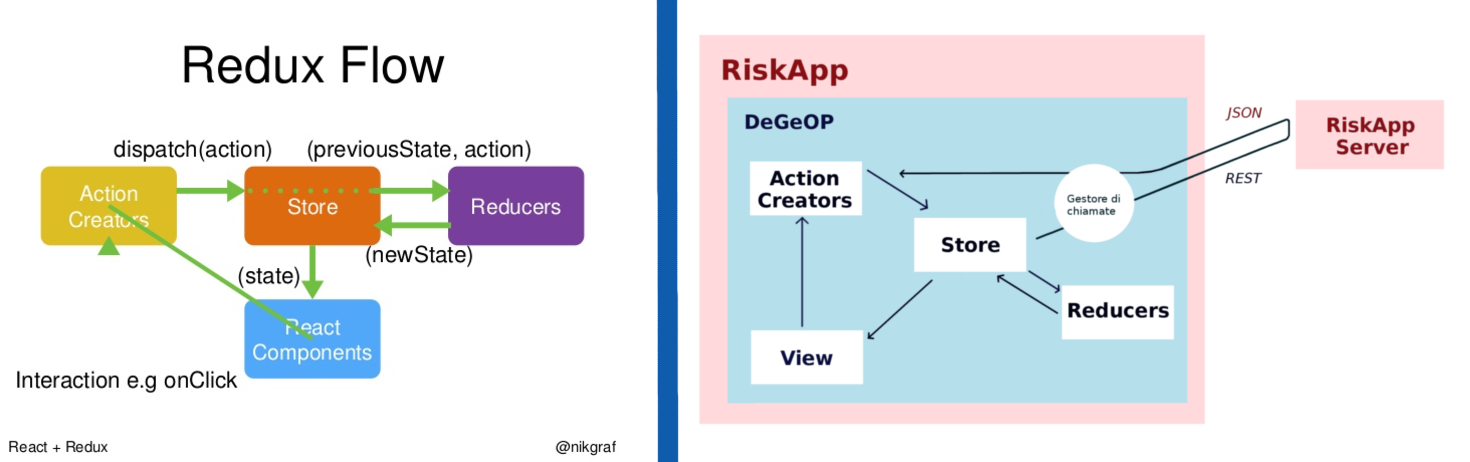
\includegraphics[scale=0.3]{img/ComparaArch.png}
		\caption{Design pattern proposto da Redux e la sua contestualizzazione in \progetto}
	\end{figure}